% REMEMBER TO SET LANGUAGE!
\documentclass[a4paper,10pt,english]{article}
\usepackage[utf8]{inputenc}
\usepackage[margin=0.5in]{geometry}
\usepackage{cite}
\usepackage{braket}
\usepackage{enumitem}
\usepackage{upgreek}
\usepackage{multicol}
\usepackage{mhchem}

% Standard stuff
\usepackage{amsmath,amsthm, amssymb,graphicx,varioref,verbatim,amsfonts,geometry,esint,url,color}
% colors in text
\usepackage[usenames,dvipsnames,svgnames,table]{xcolor}
% Hyper refs
\usepackage[colorlinks]{hyperref}
\usepackage{float}
\usepackage{wrapfig}
\usepackage{circuitikz}

\usepackage{tikz}
\usepackage[framemethod=tikz]{mdframed}
\usepackage{tikz-3dplot}
\usetikzlibrary{matrix,calc}

\usepackage{bm}

\usepackage[export]{adjustbox}

\usepackage{subfig}
\usepackage{algpseudocode}
\usepackage{algorithm}
\usepackage[makeroom]{cancel}

\usepackage{tcolorbox}
\tcbuselibrary{most}

%%%% PREVENT EXTRA WHITESPACE IN SECTION TITLES
\usepackage{sectsty}
\sectionfont{\raggedright}
%%%%

%%%%%FOR THE enumitem PACKAGE
\setlist[enumerate]{label*=\arabic*.}
%%%%%

%%%%EXAMPLE ENVIRONMENT

\newtcolorbox
[auto counter,number within=section]{pabox}[2][]{
%
enhanced,colback=black!5!white, colframe=black, fuzzy shadow={0mm}{-4pt}{-0.5pt}{0.4mm}{black!60!white},
title=Example 
\thetcbcounter
: #2,#1}

\newcommand{\example}[2]{
\begin{pabox}[label={myautocounter}]{#1}
#2
\end{pabox}
}
%%%%%%%%%%%%%%%%%%%%%%

%%%% BOX EQUATION ENVIRONMENT

\newenvironment{boxequation}{
\begin{tcolorbox}[ams equation, enhanced, colback=black!50!green!10!white, colframe=black, fuzzy shadow={0mm}{-4pt}{-0.5pt}{0.4mm}{black!60!white}]}
{\end{tcolorbox}}
%%%%%%%%%%%%%%%%%%%%%%%%%%%%%

%%%% BOX QUOTE ENVIRONMENT

\newenvironment{boxquote}{
\begin{tcolorbox}[enhanced, colback=black!50!green!10!white, colframe=black, fuzzy shadow={0mm}{-4pt}{-0.5pt}{0.4mm}{black!60!white}]
\begin{center}}
{\end{center}\end{tcolorbox}}

%%%%%%%%%%%%%%%%%%%%%%%%%%

% Document formatting
\setlength{\parindent}{0mm}
\setlength{\parskip}{1.5mm}


%Color scheme for listings
\usepackage{textcomp}
\definecolor{listinggray}{gray}{0.9}
\definecolor{lbcolor}{rgb}{0.9,0.9,0.9}

%Custom Math Operators
\DeclareMathOperator{\col}{col}
\newcommand{\colx}{\col x}

\DeclareMathOperator{\row}{row}
\newcommand{\rowx}{\row x}

\DeclareMathOperator{\nul}{nul}
\newcommand{\nulx}{\nul x}

\DeclareMathOperator{\rank}{rank}
\newcommand{\rankx}{\rank x}

\DeclareMathOperator{\Span}{span}
\newcommand{\Spanx}{\span x}

\DeclareMathOperator{\range}{range}
\newcommand{\rangex}{\range x}

\DeclareMathOperator{\dist}{dist}
\newcommand{\distx}{\dist x}

\DeclareMathOperator{\proj}{proj}
\newcommand{\projx}{\proj x}

\usepackage{listings}
\lstset{
	backgroundcolor=\color{lbcolor},
	tabsize=4,
	rulecolor=,
	language=python,
        basicstyle=\scriptsize,
        upquote=true,
        aboveskip={1.5\baselineskip},
        columns=fixed,
	numbers=left,
        showstringspaces=false,
        extendedchars=true,
        breaklines=true,
        prebreak = \raisebox{0ex}[0ex][0ex]{\ensuremath{\hookleftarrow}},
        frame=single,
        showtabs=false,
        showspaces=false,
        showstringspaces=false,
        identifierstyle=\ttfamily,
        keywordstyle=\color[rgb]{0,0,1},
        commentstyle=\color[rgb]{0.133,0.545,0.133},
        stringstyle=\color[rgb]{0.627,0.126,0.941}
        }
        
       
\newcounter{subproject}
\renewcommand{\thesubproject}{\alph{subproject}}
\newenvironment{subproj}{
\begin{description}
\item[\refstepcounter{subproject}(\thesubproject)]
}{\end{description}}


\definecolor{ubuntu_terminal_background}{RGB}{48,10,36}

\lstdefinestyle{DOS}
{
    backgroundcolor=\color{ubuntu_terminal_background},
    basicstyle=\scriptsize\color{white}\ttfamily
}

\lstnewenvironment{terminal}[1]
  {%
   \mdframed[backgroundcolor = ubuntu_terminal_background, innertopmargin = -0.4cm, innerbottommargin = -0.1cm, hidealllines = true, innerleftmargin = 0.2cm, innerrightmargin = 0.2cm]%
   \lstset{
     backgroundcolor=\color{ubuntu_terminal_background}, keywords={},
     basicstyle=\scriptsize\color{white}\ttfamily, frame = none, numbers=none
   }%
  }
  {\endmdframed}


%%%%%%%%%%%%%%  VECTORS TO BOLD
%\let\oldhat\hat
%\renewcommand{\vec}[1]{\mathbf{#1}}
%%%%%%%%%%%%%%  

%%%%%%%%%%%%%% UNIT VECTOR 
\newcommand{\uveci}{{\bm{\hat{\textnormal{\bfseries\i}}}}}
\newcommand{\uvecj}{{\bm{\hat{\textnormal{\bfseries\j}}}}}
\DeclareRobustCommand{\uvec}[1]{{%
  \ifcsname uvec#1\endcsname
     \csname uvec#1\endcsname
   \else
    \bm{\hat{\mathbf{#1}}}%
   \fi
}}
%%%%%%%%%%%%%
  
\usepackage{titlesec}

\titleformat{\chapter}[display]
  {\normalfont\bfseries\Large\raggedleft\color{black}}
  {\tikz[remember picture,overlay] \node[opacity=0.9,inner sep=0pt,anchor=north] at (current page.north){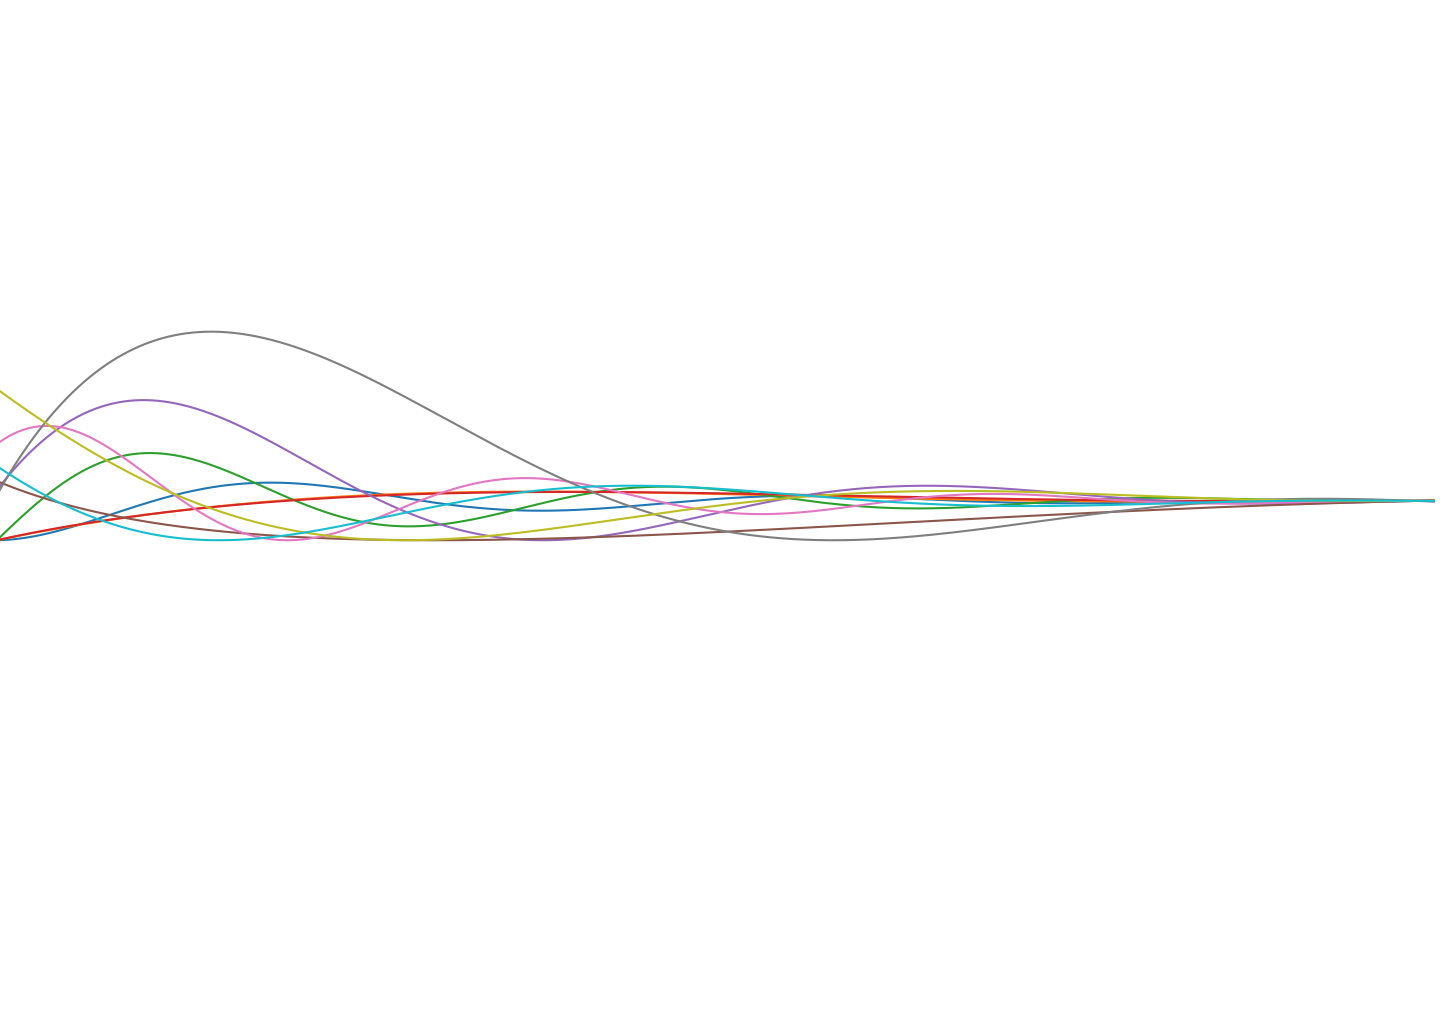
\includegraphics[width=\paperwidth,height=10cm]{header.png}};
    \MakeUppercase{\chaptertitlename}%
        \rlap{ \resizebox{!}{1.5cm}{\thechapter}}
  }
  {10pt}{\Huge}
\titlespacing*{\chapter}{0pt}{-30pt}{-5pt}

%Griffiths' style calligraphy font: use like $\scripty{r}$
\usepackage{calligra}
\DeclareMathAlphabet{\mathcalligra}{T1}{calligra}{m}{n}
\DeclareFontShape{T1}{calligra}{m}{n}{<->s*[2.2]callig15}{}
\newcommand{\scripty}[1]{\ensuremath{\mathcalligra{#1}}}

\begin{document}

\ctikzset{bipoles/length=.6cm}
\newcommand\esymbol[1]{\begin{circuitikz}
\draw (0,0) to [#1] (1,0); \end{circuitikz}}

\title{MAT4110 Mandatory Assignment 2}
\author{Gabriel Sigurd Cabrera}

\maketitle

\begin{multicols*}{2}

\section*{Premise}

We are interested in implementing the SVD – or \textit{singular value decomposition} – with the goal of compressing a set of three images, shown in Figure \ref{fig_0}:

\begin{figure}[H]
 \centering
    \subfloat[New York ($960 \times 640$ px)\label{fig_0a}]{{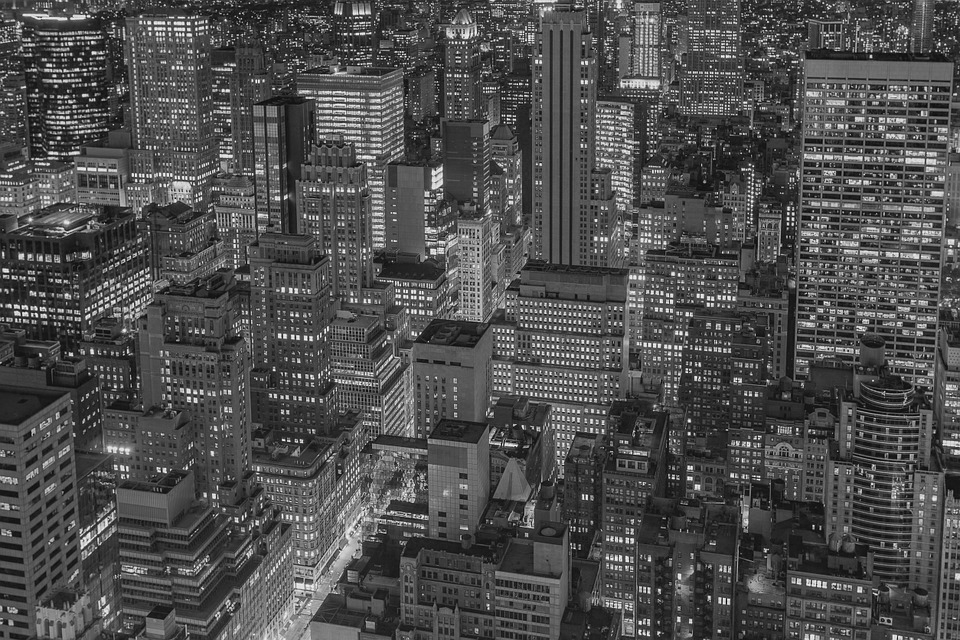
\includegraphics[width=.25\textwidth]{../New_York.png} }}
    \subfloat[Jellyfish ($960 \times 640$ px)\label{fig_0b}]{{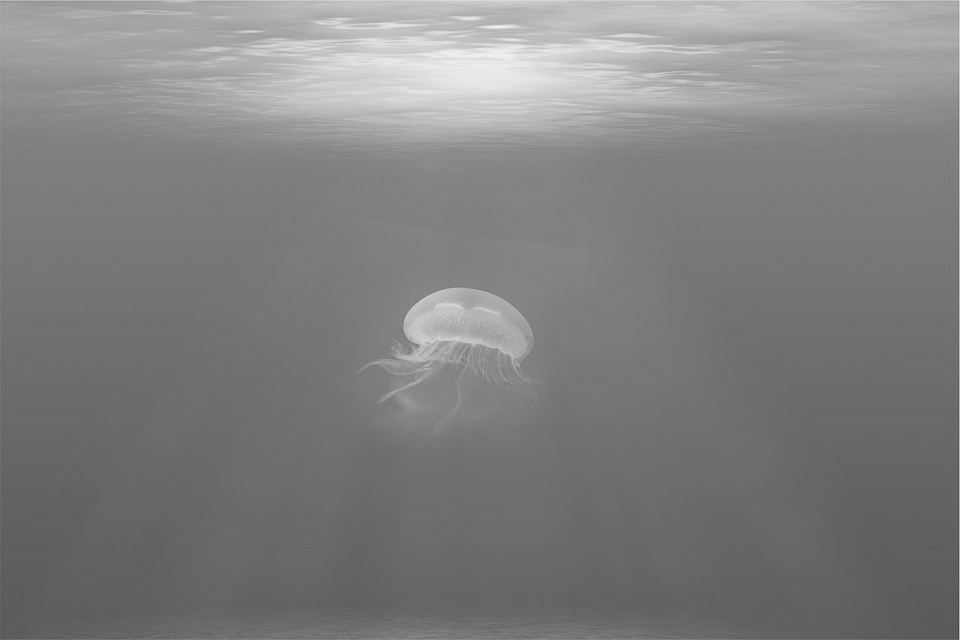
\includegraphics[width=.25\textwidth]{../Manet.png} }}
   	\qquad
    \subfloat[Chessboard ($695 \times 720$ px)\label{fig_0c}]{{
\includegraphics[width=.25\textwidth]{../Sjakkbrett.png} }}
    \caption{Three uncompressed, black and white images.\label{fig_0}}
\end{figure}

Using the \texttt{python} module \texttt{imageio}, we will represent each image as a \texttt{numpy} array of 64-bit floating-point values in the range $[0, 255]$, where $0$ is white, and $255$ is black.  

Let us call an arbitrary input array $\mathbf{X}$; since we are performing the SVD on each $\mathbf{X}$, we will use the following notation to define the SVD:

\begin{equation}
\label{eq_0}
\mathbf{U} \mathbf{\Sigma} \mathbf{V}^\textsc{t} = \mathbf{X}
\end{equation}

Where $\mathbf{X} \in \mathbb{R}^{m \times n}$, $\mathbf{U} \in \mathbb{R}^{m \times m}$, $\mathbf{\Sigma} \in \mathbb{R}^{m \times n}$, and $\mathbf{V} \in \mathbb{R}^{n \times n}$.  It is also worth noting that $\mathbf{\Sigma}$ is a \textit{diagonal matrix}; as such, we define $\mathbf{D} \equiv \text{diag}({\mathbf{\Sigma}}) = \begin{bmatrix} \sigma_1 & \sigma_2 & \cdots & \sigma_r \end{bmatrix}$

\section*{Compression}

Using the SVD to perform compression is relatively simple – one begins by implementing the decomposition as defined in (\ref{eq_0}) in order to access the singular values $\sigma_i$ given in $\mathbf{D}$.  It is by saving modified versions of $\mathbf{U}$, $\mathbf{D}$, and $\mathbf{V}$ that we intend to reduce the size of our images, though clearly we must shrink them before this becomes worthwhile, as currently this would increase our file size!

To make this process worthwhile, we have three degrees of freedom by which we can reduce our matrix size:

\begin{enumerate}
\item Reducing the number of columns in $\mathbf{U}$ and rows in $\mathbf{\Sigma}$ by an amount $\Delta m$.
\item Reducing the number of columns in $\mathbf{\Sigma}$ and columns in $\mathbf{V}$ by an amount $\Delta n$.
\item Reducing the number of singular values in $\mathbf{\Sigma}$ from $n$ to $r$.
\end{enumerate}

Since we will not be saving $\mathbf{\Sigma}$, but rather its singular values $\sigma_i$, the last item is not of much consequence.  In addition, if the number of columns in $\mathbf{U}$ or $\mathbf{V}$ are reduced, then the diagonal of $\mathbf{\Sigma}$ must also be reduced for matrix multiplication to be possible, causing $r$ to have an upper-bound defined by the shapes of $\mathbf{U}$ and $\mathbf{V}$.  Therefore, for the sake of conciseness, we will disregard the last item on our list\footnote{We will assume that the length of $\mathbf{D}$ is equal to the number of columns in $\mathbf{U}$ or $\mathbf{V}$, depending on which one is smallest.}, and focus on the first two.

Let us now define our resized matrices $\mathbf{U}^\prime \in \mathbb{R}^{m \times m - \Delta m}$, $\mathbf{\Sigma}^\prime \in \mathbb{R}^{m - \Delta m \times n - \Delta n}$, and $\mathbf{V}^\prime \in \mathbb{R}^{n \times n - \Delta n}$.  This in turn implies that $\mathbf{D}^\prime \in \mathbb{R}^{n - \Delta n}$, given the assumptions we made.

It is important to note that $\sigma_1 > \sigma_2 > \cdots > \sigma_r > 0$, since we can assign a higher significance to the largest singular values: $\mathbf{D}^\prime$ will therefore contain the first $n - \Delta n$ elements of $\mathbf{D}$.  This in turn implies that we should remove the rightmost columns of $\mathbf{U}$ and $\mathbf{V}$, when creating $\mathbf{U}^\prime$ and $\mathbf{V}^\prime$.

\subsection*{Singular Values}

Using \texttt{python} to implement the SVD for each image, we see in Figure \ref{fig_1} that the singular values decrease at rates likely dependent on the complexity of the image.

\begin{figure}[H]
 \centering
    \subfloat[New York\label{fig_1a}]{{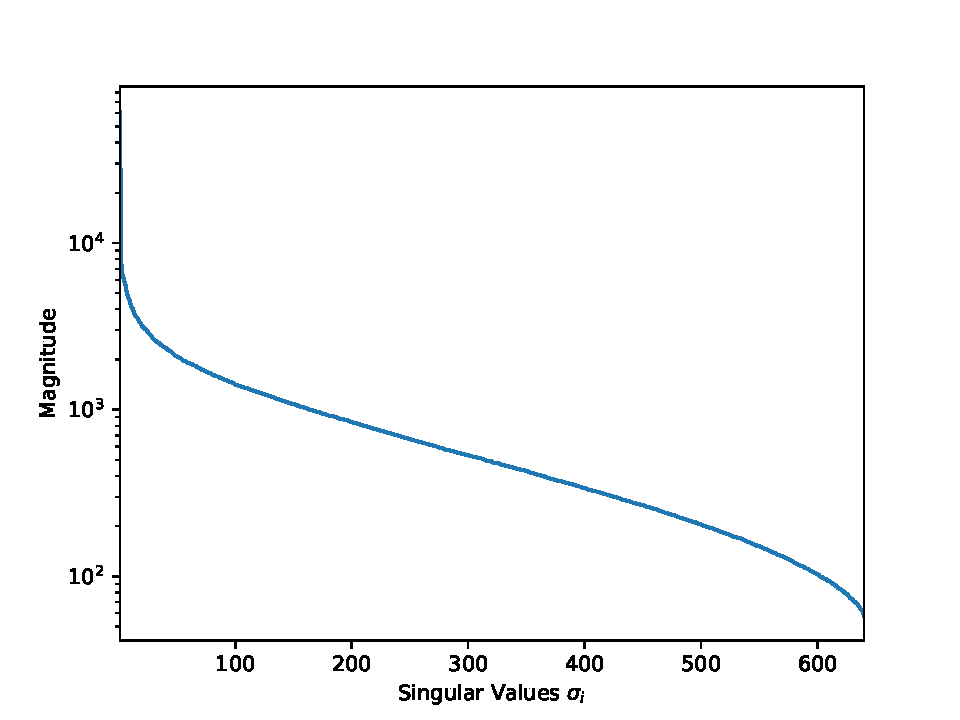
\includegraphics[width=.5\textwidth]{../singvals_0.pdf} }}
    \qquad
    \subfloat[Jellyfish\label{fig_1b}]{{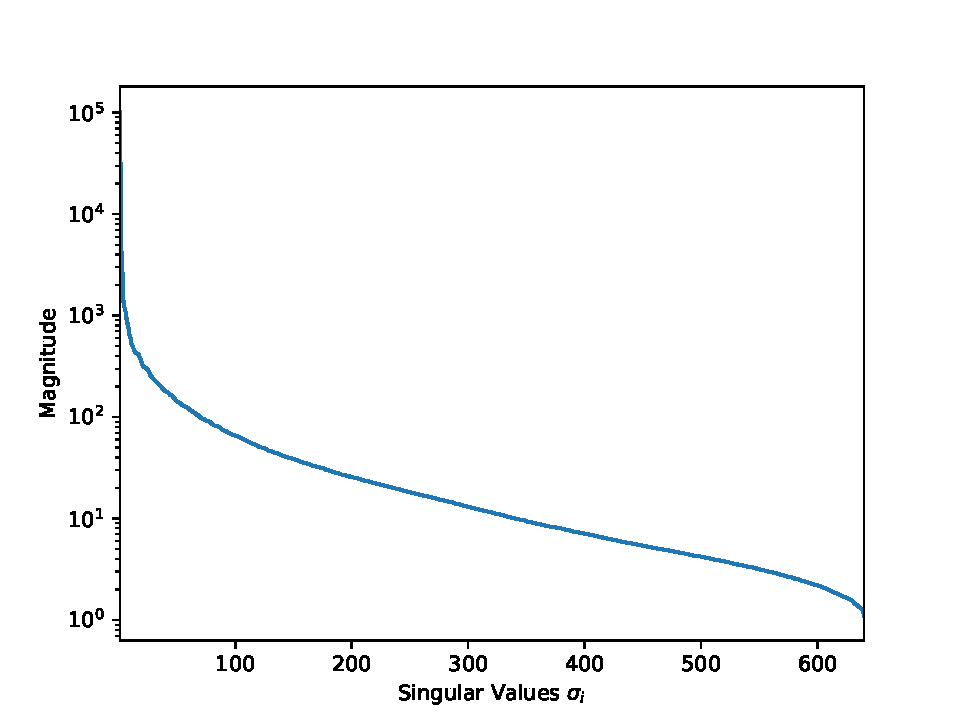
\includegraphics[width=.5\textwidth]{../singvals_1.pdf} }}
   	\qquad
    \subfloat[Chessboard\label{fig_1c}]{{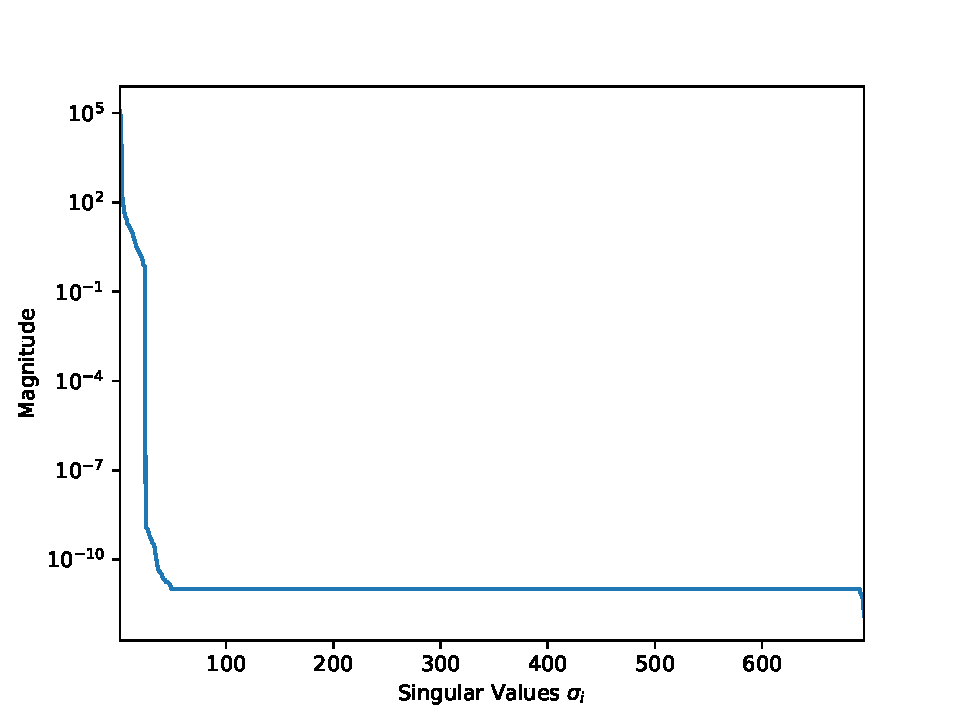
\includegraphics[width=.5\textwidth]{../singvals_2.pdf} }}
    \caption{The singular values of each decomposed image.\label{fig_1}}
\end{figure}

We see that the photographs both have very smoothly decreasing singular values (Figures \ref{fig_1a} and \ref{fig_1a}), while the computer generated chessboard has \textit{very few} large singular values (Figure \ref{fig_1c}.)  We can therefore conclude that the chessboard image will be far more compressible than the photographs, given that image quality must remain acceptable.

\subsection*{Compression Ratio}

The compression ratio $R$ is a measure of how compressed an image has become, with 1 being the uncompressed size, with a larger $R$ being more desirable than a smaller $R$.  It is defined as follows:

\begin{equation*}
R = \frac{\text{uncompressed size}}{\text{compressed size}}
\end{equation*}

By summing over the sizes of our decomposed and reduced matrices, we can represent this ratio as a function:

\begin{align*}
R(m, \Delta m, n, \Delta n, r) = \frac{mn}{m(m - \Delta m) + r + n(n - \Delta n)}
\end{align*}

Though given that $r$ is bound by our other values, it may be best to define $r \equiv \min (m - \Delta m, n - \Delta n)$, since this is the optimal value with regards to both image quality and compression effectiveness.  With this in mind, we see in Figure \ref{fig_3} how the compression ratio varies for an image the size of Figure \ref{fig_0a}:

\begin{figure}[H]
 \centering
 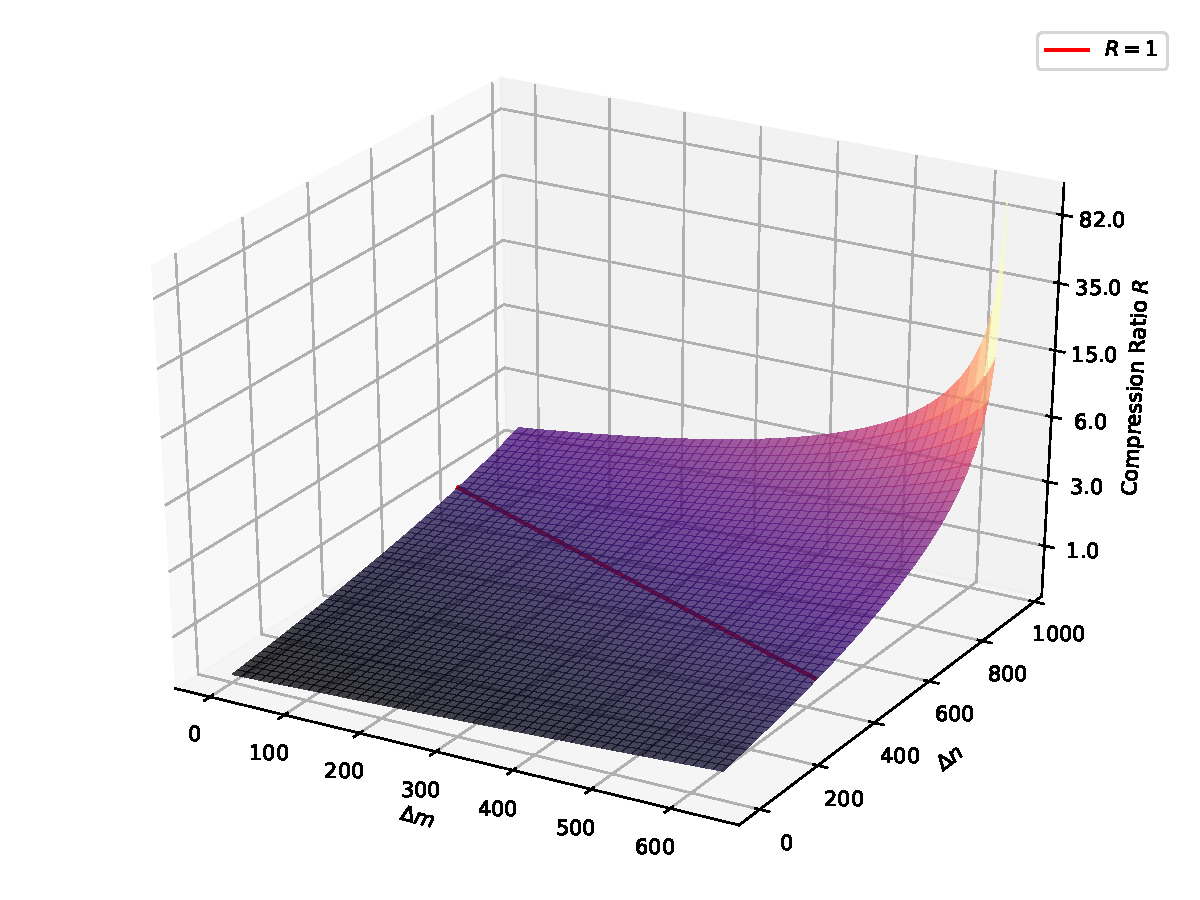
\includegraphics[width = 0.5\textwidth, center]{../comp_ratio.pdf}
 \caption{The compression ratio as a function of $\Delta m$ and $\Delta n$, with $m = 640$, $n = 960$.\label{fig_3}}
\end{figure}

It is very important to consider, however, that the \textit{image quality} is much more difficult to measure, and will require a manual analysis.

\section*{Results}

Implementing the methods aligned in the previous sections, we found that each image differed in acceptable compressability.  Through trial and error, we found the following values to be acceptable:

\begin{table}[H]
\center
\begin{tabular}{c c c c c c}
\textbf{Image} & \textbf{Label} & $\Delta m$ & $\Delta n$ & \textbf{Compression Ratio}\\
Fig. \ref{fig_0a} & New York & 330 & 700 & 1.37 \\
Fig. \ref{fig_0b} & Jellyfish & 500 & 700 & 1.81 \\
Fig. \ref{fig_0c} & Chessboard & 718 & 691 & 118.52
\end{tabular}
\caption{\label{table_0}}
\end{table}

The compressed images themselves can be seen in Figure \ref{fig_2}:
\end{multicols*}

\begin{figure}[H]
 \centering
    \subfloat[New York\label{fig_1a}]{{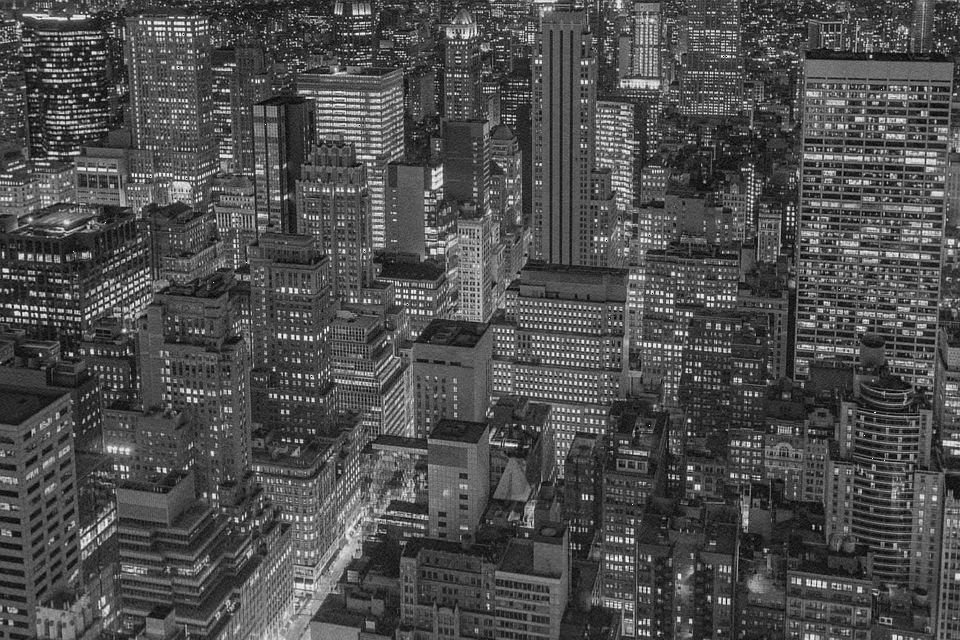
\includegraphics[width=.5\textwidth]{../New_York_compressed.png} }}
    \subfloat[Jellyfish\label{fig_1b}]{{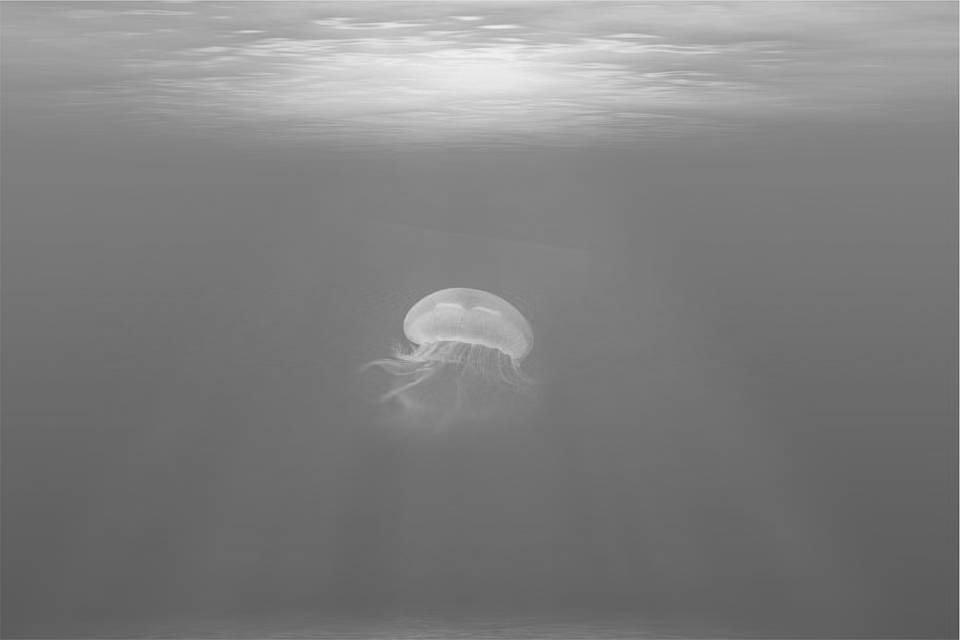
\includegraphics[width=.5\textwidth]{../Manet_compressed.png} }}
   	\qquad
    \subfloat[Chessboard\label{fig_1c}]{{
\includegraphics[width=.5\textwidth]{../Sjakkbret_compressed.png} }}
    \caption{The images from Figure \ref{fig_0}, each compressed according to the values given in Table \ref{table_0}.\label{fig_2}}
\end{figure}

We can therefore conclude that the SVD is highly effective at compressing images that are simple, such as our digitally rendered chessboard (Figure \ref{fig_0c}); we have also seen that photographs containing a lot of detail (such as Figure \ref{fig_0a}) will suffer greatly in terms of quality, with only a minor improvement in file size – less detailed photos (as in Figure \ref{fig_0b}) can be compressed slightly more effectively.

\section*{Appendix}

The script used to compress the images is available online at:

\url{https://github.com/GabrielSCabrera/MachineLearning/blob/master/MAT4110/Oblig\_2/oblig\_2.py}

\end{document}
